\documentclass{article}
\usepackage[utf8]{inputenc}
\usepackage[english]{babel}
\usepackage{amsmath}% http://ctan.org/pkg/amsmath
\usepackage{listings}
\usepackage{graphicx}
\usepackage{comment}
\usepackage{float}
\usepackage[style=ieee, backend=biber]{biblatex}
\usepackage{lscape}
\usepackage{csquotes}
\usepackage{multirow}
\addbibresource{bibliography.bib}
\usepackage[a4paper,pdftex,bottom=20mm, width=160mm]{geometry} % A4paper margins
\setlength{\parindent}{0pt} % Tar bort indenteringen på paragrafer
\setlength{\parskip}{1em}

\newcommand{\todo}[1]{\textbf{[TODO: #1]}}

\title{
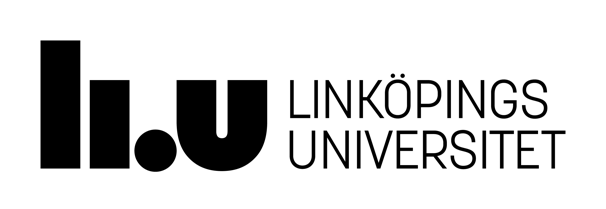
\includegraphics[scale=1.5]{liu_logga.png} \\
\vspace{2.0cm} \textbf{Planning report - The Hive G3 } \\
 \endgraf\rule{\textwidth}{.4pt}
  \large \textbf{TDDE19 Advanced Project Course - AI and Machine Learning}\\
   }


\author{
  \begin{tabular}{ccc}
    Carl Arthur     & Max Eidet       & Oscar Gustafsson \\
    \small carar002 & \small maxei163 & \small oscgu942 \\[1em]
    Jostein Tobias Melaaen & Olle Pettersson & Oskar Schrammel Rask \\
    \small josme010 & \small ollpe910 & \small osksc793 \\
  \end{tabular}
}

\date{\today}

\begin{document}

\maketitle


\newpage
\tableofcontents

\section{Introduction}
Small unmanned aerial vehicles (UAVs) are cheap, widely available and hard
to detect, which makes them a growing threat to protected assets such as
infrastructure, bases and public events. Counter-UAS (C-UAS) systems aim to
detect, classify and neutralise such drones \cite{dong2025securing}. One way
to neutralise a drone is with another drone: a defender that finds the
hostile drone with its own sensors, confirms that it is a drone and not, for
example, a bird, and then stops it.

Each step is hard. A small drone far away covers only a few pixels in a
camera image, and at that size it looks much like a bird. Once found, it
moves, so the defender has to steer towards where the target \emph{will} be,
while avoiding trees and the ground.

\section{Problem statement}
The project aims to answer two questions:
\begin{enumerate}
    \item How can a hostile drone near a protected asset be detected?
    \item How can the hostile drone be intercepted using a planning-based
          or a reinforcement-learning-based controller?
\end{enumerate}

These are broken down into three questions, each answered by one part of
the system:
\begin{itemize}
    \item \textbf{Surveillance:} how should the defenders be placed and scan
          so that a hostile drone is detected early enough to be intercepted?
          (Section~\ref{sec:base_surveillance})
    \item \textbf{Detection:} at what range, and how reliably, can the
          defenders' cameras detect a small drone and tell it apart from a
          bird? (Section~\ref{sec:detection})
    \item \textbf{Interception:} how much more often, and further from the
          base, does a predictive controller hit the target than pure
          pursuit? (Section~\ref{sec:intercept})
\end{itemize}

Each question is answered by comparing an improved method with a simple
baseline on the same scenarios, using the measures in
Section~\ref{sec:evaluation}. 

\section{Setup Overview} \label{setup_overview}
The system is developed and evaluated entirely in simulation, built on three
established open-source tools, so that the project's effort goes into
detection and interception rather than into flight control or physics.

\begin{itemize}
    \item \textbf{PX4} \cite{meier2015px4}
          is the autopilot of every drone in the simulation,
          defenders and hostile drones. It runs as software-in-the-loop,
          the same code that flies real drones, and handles stabilization,
          position control and the motors.
    \item \textbf{Gazebo} \cite{koenig2004gazebo} 
          simulates the world, the
          physics and the sensors: the military camp in a forest, the drones,
          and their cameras.
    \item \textbf{ROS~2} \cite{macenski2022ros2} 
          is the middleware that
          connects our code to PX4 and Gazebo through topics, named streams
          of messages that any program can publish to or read from.
\end{itemize}

Throughout the report, our own drones are called \emph{defenders}, and the
defender that intercepts a hostile drone is called the \emph{interceptor}.

Each drone runs its own PX4 instance in the same Gazebo world, with its own
set of ROS~2 topics. Our code reads a drone's position and state from these topics and steers it by continuously sending position or velocity setpoints, which PX4 then
flies; acceleration setpoints, which the MPC in Section~\ref{sec:intercept} needs, are planned. Camera images come from Gazebo, and the camera is pointed through PX4. Since Gazebo knows the true position of every drone, each run can also be scored against ground truth, see Section~\ref{sec:evaluation}. The whole setup runs in one Docker container, so every group member has identical software.

Our code is a Python ROS~2 package, built in layers so that the detection
and interception methods do not depend on PX4 directly:

\begin{itemize}
    \item \textbf{Drone layer:} flies one drone through PX4 and points its camera.
    \item \textbf{Swarm layer:} takes off, moves and lands several drones
          together, and places them in formations such as the ring in
          Section~\ref{sec:base_surveillance}.
    \item \textbf{Mission layer:} the components described in the following
          sections. So far it contains the interception part: a tracker that
          estimates the hostile drone's position and velocity, and the
          guidance that steers the defender. Detection and the base station will also be part of this layer.
\end{itemize}



\subsection{Assumptions}
\label{sec:assumptions}

Table~\ref{tab:assumptions} lists the assumed values of the scenario and the
platform. They hold for every system in this report, from the baseline to the
target system; additions that only the target system makes are listed in
Section~\ref{sec:target-assumptions}. The values are starting points for the
simulation and will be revised as the project progresses.

\begin{table}[H]
\centering
\small
\begin{tabular}{|l|p{0.25\textwidth}|r|p{0.27\textwidth}|}
\hline
\textbf{Symbol} & \textbf{Quantity} & \textbf{Value} & \textbf{Note} \\
\hline
$R_p$ & Perimeter radius & 1000\,m & Ring of defenders around the camp \\
$N$ & Number of defenders & varies & Derived in Section~\ref{sec:derived} \\
$h$ & Patrol altitude & 50\,m & Same for all defenders \\
$h_h$ & Hostile altitude & 20--120\,m & Range the cameras must cover \\
$v_i$ & Interceptor top speed & 12\,m/s & PX4 default \cite{px4params} \\
$v_h$ & Hostile speed & 17\,m/s & Hostile is faster than the interceptor \\
$a$ & Interceptor acceleration & 2\,m/s$^2$ & Used to reach top speed \\
$s$ & Hostile drone size & 0.5\,m & Small quadcopter \\
$\theta_0$, $W_0$, $H_0$ & Gimbal camera FOV, image size & 115$^\circ$, 1280$\times$720\,px & Camera of PX4's \texttt{x500\_gimbal} model in Gazebo \cite{px4gazebomodels}; the target system's camera is chosen in Section~\ref{sec:camera-choice} \\
$t_g$ & Gimbal turn and settle time & 0.5\,s & Per camera position \\
\hline
\end{tabular}
\caption{Assumed values of the scenario and the platform.}
\label{tab:assumptions}
\end{table}

In every scenario, the hostile drone flies a straight path towards the camp
at constant speed and altitude, and there is one hostile drone at a time.

\section{Base surveillance}\label{sec:base_surveillance}
While no threat is detected, the defenders watch the sky around the base. They must detect a hostile drone early enough for a defender to intercept it. This section presents different approaches for protecting the base.

\subsection{Baseline: static ring.} The defenders hold fixed, evenly spaced
positions in a ring. Each drone sweeps its outward sector in a fixed tempo by moving the camera, and the images are checked with the detection methods in Section~\ref{sec:detection}.

\subsection{Improvements}
When a defender leaves the ring to intercept, it leaves a gap in the
coverage. The improvement is to close this gap, which can be done in two
ways:
\begin{itemize}
    \item \textbf{Replacement:} a reserve drone is         sent out to take the
          empty position.
    \item \textbf{Redistribution:} the remaining           defenders spread out along
          the ring until they are again evenly spaced, each adjusting its
          position based only on its neighbors, as in
          \cite{kingston2008perimeter}.
\end{itemize}
Both are compared with the static baseline by the coverage lost while a
defender is away from the ring.



\newpage
\section{Drone Detection Using Sensors}
\label{sec:detection}
Detection must \emph{find} a small object in the sky, \emph{classify} it as
a drone or not, for example a bird, and give the \emph{direction} to it. A
target can be found when it covers a few pixels, but it can only be
classified reliably when it covers tens of pixels. Detection is therefore
split into a cheap first step that flags candidates and a classifier that
runs only on them.

\subsection{Sensors}
Each defender has a camera on a gimbal that scans its outward sector
(Section~\ref{sec:base_surveillance}). The baseline uses the simulated
platform's camera (Table~\ref{tab:assumptions}); the target system's camera
is chosen in Section~\ref{sec:camera-choice}.
Classification needs more pixels than detection. Johnson's criteria give
about eight pixels for recognising an object \cite{johnson1958analysis},
and a detector such as YOLO needs more in practice, so classification is
assumed to need about 20~pixels, a value that will be measured in the
simulation. By
Equation~\eqref{eq:rdet}, a camera then classifies a target at a fifth of
its detection range: about 10~m with the platform's camera and about
136~m with a 20$^\circ$ camera at 1920~px.

A thermal camera on the gimbal is an optional extension that could be tried
later: a drone's warm motors stand out against a cold sky, also at night
and against trees, where an RGB camera struggles. LiDAR is not used, since
a small drone at long range falls between the beams. A real system would
also have a radar for early warning, but Gazebo has no radar sensor.

\subsection{Baseline: Dark Object Against the Sky}
The baseline groups pixels that differ clearly from the surrounding sky
into connected regions, and reports regions of a plausible size as
candidates. It needs no training, but it cannot tell a drone from a bird
and fails when the background is not sky. Every candidate seen in $k$
consecutive images is treated as a drone.

\subsection{Improvement: YOLO26}
To detect and classify hostile drones, we will use YOLO26 from Ultralytics,
the newest version of the YOLO model family
\cite{jocher2026ultralyticsyolo26unifiedrealtime}. YOLO26 looks at an image
once and directly outputs where objects are (bounding boxes), what they are
(classes), and how confident it is, which makes it fast enough to run in
real time. Tiny drones are hard for standard YOLO models
\cite{zhai2023yolodrone}. Of YOLO26's five sizes, from nano (n) to extra
large (x), we use the two smallest, since computing power on board is
limited \cite{wang2026edge}. YOLO26n runs on
the drone, on enlarged crops of the image around the candidates, which lets
it see small targets \cite{akyon2022sahi}. YOLO26s is a candidate for the
stronger classifier at the base station (Section~\ref{sec:base-station}).

Detections are linked between images with
ByteTrack \cite{zhang2022bytetrack}, so a target keeps its identity when it
is missed in some images. A drone starts flying towards a target as soon as
YOLO26n classifies it as a drone with a confidence above $\tau$ in $k$
consecutive images (Section~\ref{sec:intercept}).

\subsection{Training Data and Fine-Tuning}
\textbf{Data collection.} Most of the training data is generated in Gazebo,
where every image can be labelled automatically. A script places drone and
bird models at random positions around a defender and points its gimbal
camera at random directions, varying the distance, altitude (20--120~m),
background (clear sky, clouds, trees and ground) and lighting. The distances
are chosen so that the targets span from a few pixels to about 100 pixels
across, with most images near the 4- and 20-pixel limits that matter for
detection and classification. Each object's bounding box is computed from
its true position and the camera's pose, or read directly from Gazebo's
bounding-box camera sensor, which also handles objects hidden behind trees.
Images with no drone or bird are included as well, so that the model learns
to ignore clouds and trees. The images are split into training, validation
and test sets by simulation run rather than by image, since consecutive
images from the same run are nearly identical and would otherwise make the
test results look better than they are.

\textbf{Fine-tuning.} Training starts from Ultralytics' YOLO26n and YOLO26s
weights pretrained on COCO, whose backbones already extract general visual
features. The classification part of the detection head, which for COCO has
one output per each of 80 classes, is replaced with one that has only two
outputs, \emph{drone} and \emph{bird}, and is trained from scratch, while the
rest of the network keeps its pretrained weights. Everything else in an image,
such as clouds, trees and buildings, is treated as background, so the model
learns to ignore it from the training images. Training is done in two steps.
First, the models are fine-tuned on the Seraphim drone dataset
\cite{seraphim}, about 83\,000 real drone images, so that they learn what
drones look like in many settings. Second, they are fine-tuned on the Gazebo
images, with part of the Seraphim images mixed in so that the models do not
forget them. The Drone-vs-Bird dataset \cite{coluccia2021drone}, real
videos of small drones with birds as distractors, could be added if birds
turn out to be hard to reject. Since YOLO26n runs on crops of the camera
image, it is trained on crops of the same size, so that a target has the
same size in pixels during training as during use \cite{akyon2022sahi}.
Training runs on a GPU with the standard Ultralytics augmentations, such as
changes in brightness and scale, and stops when the result on the validation
set no longer improves. The confidence threshold $\tau$ is then chosen on
the validation set so that almost no drones are missed. All results are
reported on a test set of held-out Gazebo runs, since the system has to
perform in the simulation.

\subsection{Direction and Identification}
The centre of a bounding box gives the direction to the target, from the
camera's intrinsic parameters and the gimbal's orientation
\cite{hartley2004multiple}. One camera does not measure the range, but the
width of the box gives a rough estimate: assuming the target has the size
$s$ in Table~\ref{tab:assumptions}, a target that covers $p$ pixels is at
range $r \approx f s / p$, as in Equation~\eqref{eq:rdet}. This estimate is
uncertain, since the hostile drone's true size is unknown and an error of
one pixel is a large part of a target only a few pixels wide. The drone
therefore sends the base station an estimated position together with its
uncertainty, which is small across the line of sight and large along it.
The base station's Kalman filter combines these estimates with those of
other drones (Section~\ref{sec:base-station}). Once two or more drones see
the target, triangulation (Equation~\eqref{eq:triangulation}) gives an
accurate position; until then, the single-drone estimate fills the gap.
The base station also knows every defender's position from its telemetry,
so a detection within a few metres of a defender's reported position is
classified as friendly. Only the remaining detections can be hostile.

\subsection{Evaluation}
The dark-object baseline and YOLO26 are compared on the same seeded
scenarios, in which a hostile drone and birds approach the base from random
directions. A detection counts as correct if its centre lies within a few
pixels of the target's true position projected into the image, since box
overlap is unstable for targets only a few pixels wide. The measures are:
\begin{itemize}
    \item \textbf{Missed drones:} the share of hostile drones that reach the
          ring undetected, the most important measure.
    \item \textbf{Detection probability versus range:} the share of hostile
          drones detected in each range interval, which shows where detection
          starts to fail.
    \item \textbf{Birds flagged as drones:} the share of birds seen by a
          camera that are classified as drones.
    \item \textbf{Background false alarms:} detections of drones in images
          with no drone or bird, per image.
    \item \textbf{Recall versus target size:} the share of drones detected in
          held-out Gazebo images, grouped by their size in pixels, which tests
          the assumptions of 4 pixels for detection and 20 pixels for
          classification.
    \item \textbf{Inference time} of YOLO26n and YOLO26s per image on a CPU.
\end{itemize}


\subsection{Interface}
\label{sec:detection-interface}
The detection component produces one \emph{detection report} for each
target it follows (Table~\ref{tab:detection-report}). The report is used
in three places: on the drone, every image, by the gimbal controller and
the guidance law (Section~\ref{sec:intercept}); by the scan, which stops
when a target is found (Section~\ref{sec:base_surveillance}); and at the
base station, every $\Delta t$ (Section~\ref{sec:target-assumptions}),
together with an image crop of the target (Section~\ref{sec:base-station}).

\begin{table}[H]
\centering
\small
\begin{tabular}{|l|p{0.62\textwidth}|}
\hline
\textbf{Field} & \textbf{Content} \\
\hline
Time & When the image was taken \\
Drone & Which drone saw the target \\
Track & Identity of the target over time, from ByteTrack \\
Stage & \emph{Candidate} (first step) or \emph{classified} (YOLO26) \\
Class and confidence & \emph{Drone} or \emph{bird}, with the model's confidence \\
Direction & Unit vector from the drone to the target, in the world frame,
            with its uncertainty \\
Range & Rough range from the target's size in the image, with its
        uncertainty \\
Bounding box & Position and size in pixels; used only on the drone, to
               centre the target in the image \\
\hline
\end{tabular}
\caption{Contents of a detection report (draft).}
\label{tab:detection-report}
\end{table}

The direction is given in the world frame rather than in pixels, so that
the components that use it do not depend on which camera is chosen
(Section~\ref{sec:camera-choice}). Direction and range are kept apart
rather than combined into a single position, since the direction is
accurate while the range is not, and the guidance laws need only the
direction. Whether a detection is a friendly drone is decided at the base
station, which knows every defender's position, and is therefore not part
of the report.
% TODO: decide message format (e.g. a custom ROS 2 message or
% vision_msgs/Detection2DArray), the rate on the drone, and how the
% uncertainties are represented.
\section{Base Station}
\label{sec:base-station}

The base station sits between detection on the drones
(Section~\ref{sec:detection}) and interception (Section~\ref{sec:intercept}).
It does not fly and has no camera of its own; it works on what the drones send
it. A drone that detects an object starts flying towards it at once and, during
its flight, sends image crops of the object and the direction to it every
$\Delta t$ seconds (Section~\ref{sec:target}). The base station sees the
reports of every drone at the same time, which no single drone does. This
section describes what the base station could do with them.

\textbf{Confirming the target.} The base station could run a stronger
classifier than the one on the drones, since it is not limited by the drones'
weight and power. Instead of one image, it could classify the sequence of
crops a drone sends, in which motion and shape over time help to tell a drone
from a bird, and combine the views of several drones that see the same
object. Since missing a hostile drone is worse than a detour, it would be
tuned so that it rarely misses a drone, and call a drone back only when it is
confident that the object is not a drone.

\textbf{Estimating the target's position.} One camera gives only the direction
to the target, not its distance. With the directions from two drones, the
base station could estimate the target's position by triangulation. Two
drones at positions $\mathbf{p}_1$ and $\mathbf{p}_2$ see the target along unit
directions $\mathbf{u}_1$ and $\mathbf{u}_2$; since the two lines rarely meet
exactly, one option is the midpoint of their closest points, the classic
midpoint method \cite{hartley1997triangulation, hartley2004multiple},
\begin{equation}
  \hat{\mathbf{x}} = \tfrac{1}{2}\left(\mathbf{p}_1 + s^\ast\mathbf{u}_1
                   + \mathbf{p}_2 + t^\ast\mathbf{u}_2\right),
  \quad
  (s^\ast, t^\ast) = \arg\min_{s,t}
  \left\|\mathbf{p}_1 + s\,\mathbf{u}_1 - \mathbf{p}_2 - t\,\mathbf{u}_2\right\|^2 .
  \label{eq:triangulation}
\end{equation}
A Kalman filter could smooth the estimates over time and give the target's
velocity as well, which the MPC in Section~\ref{sec:intercept} needs, with new
directions matched to the track by, for example, the nearest-neighbour rule
\cite{barshalom2001estimation}. With more drones seeing the target, the
estimate could use all of their directions.

\textbf{Choosing the drones.} The base station could decide which drones take
part in an intercept: confirming the drone that is already on its way, and
sending a second drone so that the target can be triangulated. It could pick
the drones that can reach the hostile drone's path earliest, for example with
a consensus-based auction between the drones \cite{choi2009consensus}.

\section{Interception}\label{sec:intercept}
Interception starts when an object has been detected as a drone. In the
baseline, this is when the detector's confidence exceeds a threshold $\tau$
in $k$ consecutive images. In the target system, the interceptor starts
flying at the first detection by the drone's own model, and the base station
confirms the target or calls the interceptor back while it flies
(Section~\ref{sec:base-station}). The centre of the bounding box is converted
into a direction to the target, using the camera's intrinsic parameters and
the gimbal's orientation, as in \cite{zheng2025mcm}. Two PID controllers turn
the gimbal so that the target stays in the centre of the image, and a Kalman
filter smooths the direction, estimates how fast it turns, and predicts it
when the target is briefly lost. The gimbal loop must react fast enough to
keep the target in view: by Equation~\eqref{eq:angrate}, a target crossing at
17\,m/s leaves a 20$^\circ$ view within about 0.2\,s at 20\,m if the gimbal
lags. This is one reason the target system considers a wide view on the
gimbal for close range (Section~\ref{sec:camera-choice}).

\subsection{Guidance Laws}

Three guidance laws are compared. Pure pursuit and proportional navigation
need only the direction to the target and its rate of change, which one
camera provides; the MPC also needs the target's position and velocity, which
one camera measures poorly.

\textbf{Baseline: pure pursuit.} The interceptor flies at full speed towards
the target's current direction, while the gimbal keeps the target in the
centre of the image. Its weakness is that it always aims at where the target
\emph{is}, not where it is going, so against a crossing or turning target it
ends up behind the target and has to chase it. It can therefore only catch a
target that is slower than itself: against a hostile drone faster than $v_i$
(Table~\ref{tab:assumptions}), it falls behind and never hits.

\textbf{Target system: MPC.} The interceptor uses the MPC of Zheng et al.\
\cite{zheng2025mcm}. It predicts the target's trajectory over $K$ steps from
its estimated position and velocity, assuming constant velocity, and chooses
the accelerations $\mathbf{u}(k)$ that minimise
\begin{equation}
  J = \sum_{k=1}^{K} \|\mathbf{p}_{\mathrm{exp}}(k) - \mathbf{p}(k)\|^2_{Q}
      + \|\mathbf{u}(k)\|^2_{R},
\end{equation}
where $\mathbf{p}_{\mathrm{exp}}$ is the target's predicted position and
$\mathbf{p}$ the interceptor's. The problem has an analytical solution; the
first acceleration is sent to PX4 and the problem is solved again at the next
step. Unlike \cite{zheng2025mcm}, who keep an offset around the target to fire
a net, the offset here is zero. Since the hostile drone does not always fly
in a straight line, the constant-velocity prediction is wrong when it turns,
but it is corrected at every step as new estimates arrive; Zheng et al.\
used the same model against a target flying in a circle. The MPC needs the
target's position and velocity, which one camera cannot give. It is therefore
only possible with triangulation from two or more defenders, for which the
base station sends a second defender (Section~\ref{sec:base-station}), and is part of
the target system.

\subsection{Evaluation}
Metrics are computed by the scenario runner from the true positions in
Gazebo, never from the interceptor's estimates. The target always flies
towards the base, and a run ends with a \emph{hit} (interceptor within
1.5\,m of the target), the \emph{target reaching the base}, the \emph{target
being lost}, or a \emph{timeout}. Head-on, the two drones close at up to
$v_i + v_h \approx 29$\,m/s, about 2.9\,m between two samples at 10\,Hz, which
is more than the hit radius. The closest distance is therefore computed along
the straight line between consecutive samples, not only at the samples.

\textbf{Alternative success: lock-on.} How the hostile drone is finally
stopped is outside the scope of this project, and flying into it is only one
option. An interception may therefore also be counted as successful when the
interceptor holds a \emph{lock-on} on the hostile drone for $t_{\mathrm{lock}}$
seconds. The interceptor has a lock-on when the target is inside its gimbal
camera's view, the detector confirms it as a drone in at least $k$ of every
$n$ consecutive images, and the interceptor is within a distance
$d_{\mathrm{lock}}$ of it. The lock-on must last $t_{\mathrm{lock}}$ seconds
without a break, and be held before the target comes within $x$\,m of its
goal (Section~\ref{sec:evaluation}). A sustained lock-on shows that the
interceptor could follow and engage the target with whatever means is chosen
later. The assumed values of $t_{\mathrm{lock}}$ and $d_{\mathrm{lock}}$ are
listed in Table~\ref{tab:target-assumptions}; both success criteria are
reported for every run.

For each run the following are recorded:

\begin{itemize}
    \item \textbf{Hit or not:} Whether the interceptor successfully intercepted the target.
    \item \textbf{Time to hit:} The time elapsed from first detection to interception.
    \item \textbf{Lock-on:} Whether a lock-on was held for $t_{\mathrm{lock}}$ seconds, the time from first detection until it started, and the longest unbroken lock-on in the run.
    \item \textbf{Distance to base at hit:} How far the target was from the protected asset when neutralized.
    \item \textbf{Target's closest distance to base:} A measure of how close the threat got before being stopped.
    \item \textbf{Closest distance between interceptor and target:} Useful for evaluating near-misses in unsuccessful runs.
\end{itemize}

All methods are run on the same seeded scenarios: a target approaching
head-on and crossing at 30, 60 and 90$^\circ$, at increasing speeds from
4\,m/s up to and beyond the interceptor's top speed $v_i$, including the
hostile speed $v_h$ of Table~\ref{tab:assumptions}, each 30--50 times. Each
method is run both with YOLO detections and with perfect detections from the
true position, which separates errors in guidance from errors in detection.
The measured time to hit is also compared with the margins predicted in
Table~\ref{tab:feasibility}, which tests the analysis in
Section~\ref{sec:derived}. When the target is lost, another drone that still
sees it could take over; this is not evaluated here.

Since the sensors have not yet been tested, realistic distances and speeds
are not known. Zheng et al.\ \cite{zheng2025mcm} captured a target moving at
4~m/s in 64.7\% of their outdoor attempts. The project aims for a similar
share of hits. Pure pursuit is expected to hit only while the target is
slower than $v_i$; proportional navigation and the MPC are expected to hit
more often, earlier and further from the base.
\section{Baseline System}\label{sec:baseline}
The baseline system is the simplest complete version of the system, built
from the simplest method in each component. Every later method is evaluated
on the same scenarios and compared against it. In each run, a hostile drone spawns at a random location far from the base, with the goal of flying to the military camp in the center of the world. The defender drones are deployed to the formation described in Section~\ref{sec:base_surveillance} and scan the surrounding area with their gimbal cameras. When a defender detects the hostile drone, the detection and classification component decides whether it is a drone. If it is, the defender intercepts it by flying into it.

\section{Target System}\label{sec:target}
%% Oscar Gustafsson

In the target system, a ring of $N$ friendly drones patrols at radius $R_p$
around a protected military camp. Each drone carries a camera on a gimbal
that scans the sky outside the ring; which camera, and whether a second one
is added, is chosen in Section~\ref{sec:camera-choice}. A hostile drone
approaches from outside at speed $v_h$. The nearest friendly drone sees it as
a small dark object against the sky. A fast model on the drone flags the
object, and the drone starts flying towards it at once, without waiting for
the base station. Throughout its flight, it sends an image crop of the object
and the direction to it every $\Delta t$ seconds. The base station acts on
these (Section~\ref{sec:base-station}): a stronger model classifies the
object, and if it is a drone, the base station confirms the intercept and
sends a second drone so that the target can be triangulated; if it is not,
the base station calls the drone back. Since missing a hostile drone is worse
than a detour, the drone is only called back when the base station is
confident that the object is not a drone. The interceptor acquires and locks
on to the target, keeps it centred in its gimbal camera, and guides itself to
the intercept. All
numbers below follow from the assumptions in Section~\ref{sec:assumptions} and
Section~\ref{sec:target-assumptions}; when an assumption changes, the derived
values change with it.

\subsection{Additional Assumptions}
\label{sec:target-assumptions}

The target system adds components and constraints that the baseline does not
have. Table~\ref{tab:target-assumptions} lists their assumed values, on top of
those in Table~\ref{tab:assumptions}.

\begin{table}[H]
\centering
\small
\begin{tabular}{|l|p{0.25\textwidth}|r|p{0.27\textwidth}|}
\hline
\textbf{Symbol} & \textbf{Quantity} & \textbf{Value} & \textbf{Note} \\
\hline
$\Theta_s$ & Sector scanned by the gimbal camera & 180$^\circ$ & Constraint: outward half only, since threats come from outside \\
$\Delta t$ & Interval between image crops sent to the base station & 0.2\,s & Addition: 5 crops per second \\
$t_c$ & Image sequence needed to classify & 1.0\,s & Addition: base-station classifier, $t_c/\Delta t = 5$ crops \\
$t_l$ & Radio link and inference latency & 0.1\,s & Addition: drone to base station and back \\
$p_{\min}$ & Smallest detectable size & 4\,px & Analysis: dark object against the sky \\
$t_{\mathrm{lock}}$ & Lock-on time that counts as a successful interception & 3\,s & Evaluation: alternative to a hit (Section~\ref{sec:intercept}) \\
$d_{\mathrm{lock}}$ & Largest distance for a lock-on & 20\,m & Evaluation: close enough to engage the target \\
\hline
\end{tabular}
\caption{Additional assumed values of the target system.}
\label{tab:target-assumptions}
\end{table}

By Johnson's criteria, detecting that an object is present needs about one
line pair, that is two pixels, across it \cite{johnson1958analysis};
$p_{\min} = 4$\,px doubles that as a margin. For the analysis below, a camera
is also assumed to detect the target as soon as it is at least $p_{\min}$
pixels wide, images have a 16:9 aspect ratio, and
the ring is treated as locally straight where the hostile drone crosses it.
The camera's field of view $\theta$ and image width $W$ are left open; they
are the design variables of Section~\ref{sec:camera-choice}.

\subsection{Derived Quantities}
\label{sec:derived}

\textbf{Drone spacing (sparsity).} With $N$ drones evenly spaced on the ring,
the distance between neighbours is
\begin{equation}
  d = \frac{2\pi R_p}{N},
  \label{eq:spacing}
\end{equation}
and a hostile drone that crosses the ring midway between two neighbours passes
at a lateral distance of at most
\begin{equation}
  y_{\max} = \frac{d}{2} = \frac{\pi R_p}{N}
  \label{eq:ymax}
\end{equation}
from the nearest friendly drone.

\textbf{Detection range.} By the pinhole camera model
\cite{hartley2004multiple}, a camera of width $W$ pixels and horizontal field
of view $\theta$ has a focal length, in pixels, of
\begin{equation}
  f = \frac{W/2}{\tan(\theta/2)}.
  \label{eq:focal}
\end{equation}
A target of size $s$ at range $r$ covers $p = f s / r$ pixels, so the
detection range is
\begin{equation}
  r_{\mathrm{det}} = \frac{f\,s}{p_{\min}}.
  \label{eq:rdet}
\end{equation}

\textbf{Coverage without gaps.} Every hostile drone that crosses the ring is
seen if $r_{\mathrm{det}} \geq y_{\max}$, which by Equation~\eqref{eq:ymax}
requires
\begin{equation}
  N \geq \left\lceil \frac{\pi R_p}{r_{\mathrm{det}}} \right\rceil.
  \label{eq:ncoverage}
\end{equation}

\textbf{Scanning.} A camera with image size $W \times H$ has the vertical field
of view
\begin{equation}
  \theta_v = 2\arctan\!\left(\tan\frac{\theta}{2}\cdot\frac{H}{W}\right).
  \label{eq:vfov}
\end{equation}
At range $r_{\mathrm{det}}$, hostile altitudes between $h_{h,\min}$ and
$h_{h,\max}$ span the elevation band
$\Delta\varepsilon = \arctan\frac{h_{h,\max}-h}{r_{\mathrm{det}}}
 - \arctan\frac{h_{h,\min}-h}{r_{\mathrm{det}}}$.
Covering the outward sector $\Theta_s$ then takes
$n = \lceil \Theta_s/\theta \rceil \cdot \lceil \Delta\varepsilon/\theta_v \rceil$
camera positions, and one sweep takes
\begin{equation}
  T_{\mathrm{sweep}} = n\,t_g ,
  \label{eq:sweep}
\end{equation}
during which the hostile drone flies $v_h T_{\mathrm{sweep}}$.

\textbf{Time to depart.} In the worst case, the hostile drone enters the
detection range just after the camera has looked past it. The drone that
detects it starts flying as soon as its own model flags the object, so the
time from entering detection range to departure is
\begin{equation}
  t_d = T_{\mathrm{sweep}} + t_g .
  \label{eq:delay}
\end{equation}
The base station's decision arrives $t_c + t_l$ later, while the drone is
already on its way, so it does not delay the intercept; it only decides
whether the flight continues.

\textbf{Intercept feasibility.} Since $v_h > v_i$, the interceptor cannot catch
the hostile drone from behind; it must reach the hostile drone's path before
the hostile drone gets there. Conservatively, the meeting point is where the
hostile drone crosses the ring. A hostile drone first detected at range
$r_{\mathrm{det}}$ by a drone at lateral distance $y$ reaches the ring after
\begin{equation}
  t_h = \frac{\sqrt{r_{\mathrm{det}}^2 - y^2}}{v_h},
  \label{eq:th}
\end{equation}
and the interceptor reaches the hostile drone's path after
\begin{equation}
  t_i = t_d + \frac{y}{v_i} + \frac{v_i}{2a},
  \label{eq:ti}
\end{equation}
where the last term is the time lost while accelerating to $v_i$. The
intercept is feasible when $t_h \geq t_i$ at the worst case $y = y_{\max}$.

\textbf{Keeping the target in view.} A target that moves across the line of
sight at speed $v_\perp$ and range $r$ turns, as seen by the camera, at the
rate
\begin{equation}
  \omega = \frac{v_\perp}{r},
  \label{eq:angrate}
\end{equation}
and leaves the image after $(\theta/2)/\omega$ if the gimbal stops following
it.

\subsection{Camera Choice}
\label{sec:camera-choice}

The camera is a trade-off. A narrower field of view or a wider image raises
the focal length (Equation~\eqref{eq:focal}) and so the detection range, but a
narrower field of view needs more camera positions to scan the sector, which
lengthens the sweep and the time to decide. Table~\ref{tab:coverage} shows the
effect on the number of drones for a range of cameras, including the one the
simulated platform already has.

\begin{table}[H]
\centering
\small
\begin{tabular}{|r|r|r|r|r|r|r|}
\hline
$\theta$ & $W$ (px) & $r_{\mathrm{det}}$ & Positions $n$ & $T_{\mathrm{sweep}}$ & $N$, no gaps & $N$, feasible \\
\hline
115$^\circ$ & 1280 & 51\,m   & 4  & 2.0\,s & 62 & -- \\
115$^\circ$ & 3840 & 153\,m  & 2  & 1.0\,s & 21 & 65 \\
60$^\circ$  & 1920 & 208\,m  & 3  & 1.5\,s & 16 & 42 \\
30$^\circ$  & 1920 & 448\,m  & 6  & 3.0\,s & 8  & 16 \\
20$^\circ$  & 1920 & 681\,m  & 9  & 4.5\,s & 5  & 10 \\
10$^\circ$  & 1920 & 1372\,m & 18 & 9.0\,s & 3  & 5 \\
20$^\circ$  & 3840 & 1361\,m & 9  & 4.5\,s & 3  & 5 \\
\hline
\end{tabular}
\caption{Detection range, scan time and the number of drones needed, from
Equations~\eqref{eq:spacing}--\eqref{eq:ti}. The first row is the camera of
the simulated platform (Table~\ref{tab:assumptions}); -- means that no number
of drones makes the intercept feasible.}
\label{tab:coverage}
\end{table}

Three conclusions follow.

\textbf{The platform's camera is not enough.} With the camera of the simulated
platform, a 0.5\,m drone is detectable at only about 51\,m, and no number of
drones on a 1\,km ring makes the intercept feasible. The target system
therefore needs a camera with a longer focal length than the simulation's
default.

\textbf{Within the model, narrower is better, with diminishing returns.} At
1920\,px, going from 60$^\circ$ to 20$^\circ$ cuts the drones needed from 42
to 10; going further to 10$^\circ$ saves only five more. The model
does not limit how narrow the camera can be, so the limit must come from what
it leaves out:
\begin{itemize}
  \item \emph{Keeping the target in view.} By Equation~\eqref{eq:angrate}, a
        target crossing at 17\,m/s turns at about 19.5$^\circ$/s at 50\,m and
        49$^\circ$/s at 20\,m. A 20$^\circ$ camera loses it after about
        0.2\,s at 20\,m if the gimbal lags; a 115$^\circ$ camera keeps it for
        about 1.2\,s. A narrow camera is good for finding the target far away
        but poor for keeping it close in.
  \item \emph{Computing cost.} The detector's work grows with the number of
        pixels: a 1920$\times$1080 image has 2.25 times, and a
        3840$\times$2160 image 9 times, the pixels of the platform's
        1280$\times$720 image. This matters on board the drone and when many
        drones render cameras in the same simulation.
  \item \emph{Pointing and stabilisation.} The narrower the camera, the more
        precisely the gimbal must point and hold still; a pointing error of
        half the field of view already loses the target.
\end{itemize}

\textbf{Options to test.} These effects are not known well enough to fix the
camera now. The target system is therefore evaluated in simulation with the
following options, using the platform's camera as the reference:
\begin{enumerate}
  \item \emph{One narrower gimbal camera}, about 20--30$^\circ$ at 1920\,px:
        the simplest option that makes the intercept feasible
        (Table~\ref{tab:coverage}).
  \item \emph{A narrow and a wide camera on the same gimbal}, or a zoom
        camera, which is wide when close and narrow when far: the narrow view
        finds the target far away, and the wide view keeps it in view at
        close range, where Equation~\eqref{eq:angrate} shows the narrow
        camera struggles. The wide view also shows where to turn the gimbal
        so that the narrow camera sees an object (\emph{slew-to-cue}), as in
        master--slave surveillance systems where a wide camera directs a
        pan--tilt--zoom camera \cite{delbimbo2010exploiting}. In Gazebo, both
        variants can be built as two camera sensors on the gimbal.
  \item \emph{Several narrow cameras side by side} (a camera array): nine
        20$^\circ$ cameras cover the 180$^\circ$ sector at once, so no
        scanning is needed and $T_{\mathrm{sweep}}$ disappears. Once a target
        is detected, lock-on needs only the one camera that sees it. The gain
        is smaller than it seems, because most of the intercept time is the
        flight, not the search: with $t_d \approx 0$, the minimum number of
        drones falls from 10 to 9, and the margin with 12 drones grows from
        7\,s to 12\,s. Three costs come with it:
        \begin{itemize}
          \item \emph{Detection runs on every camera.} Until something is
                found, all cameras must be searched: nine 1920$\times$1080
                images are 20 times the pixels of the platform's camera per
                frame. Processing them in turn at 30 images per second keeps
                the computing cost of one camera and still gives a cycle of
                0.3\,s, which leaves the minimum at 9 drones.
          \item \emph{The array tilts with the drone.} Fixed to the drone, the
                cameras pitch with it (Equation~\eqref{eq:tilt}); with a
                vertical field of view of only 11.3$^\circ$, covering a pitch
                of $\pm15^\circ$ takes four rows, that is 36 cameras. The
                array must therefore be stabilised, for example on a gimbal,
                which then carries nine cameras instead of one.
          \item \emph{Weight, power and simulation.} Every camera adds weight,
                power and bandwidth on a real drone, and rendering time in
                Gazebo, multiplied by the number of drones.
        \end{itemize}
\end{enumerate}
The option that intercepts most often with the fewest drones is chosen. Until
then, the analysis uses 20$^\circ$ at 1920\,px as its example.

\textbf{Rejected: a wide camera fixed to the drone.} A multirotor tilts to
accelerate: holding its altitude while accelerating horizontally at $a$, it
pitches by
\begin{equation}
  \phi = \arctan\frac{a}{g},
  \label{eq:tilt}
\end{equation}
where $g$ is the gravitational acceleration; $a = 2$\,m/s$^2$ already gives
$\phi \approx 11.5^\circ$. It tilts further when it brakes, turns or flies into wind. A camera fixed to the
drone tilts with it, so a target at elevation $\varepsilon$ above the horizon
stays in view only if
\begin{equation}
  \varepsilon + \phi \leq \frac{\theta_v}{2}.
  \label{eq:tiltview}
\end{equation}
Even a 115$^\circ$ camera, with $\theta_v \approx 83^\circ$, keeps only
targets less than 11.5$^\circ$ above the horizon in view at a pitch of
30$^\circ$, and the image shifts every time the drone changes its attitude.
This happens exactly during the intercept, when the drone accelerates hardest
and the target is close and high in the image. A gimbal removes the drone's
pitch, so all cameras of the target system are mounted on the gimbal.

\textbf{Example: 20$^\circ$ at 1920\,px.} The camera's vertical field of view
is 11.3$^\circ$ (Equation~\eqref{eq:vfov}). At $r_{\mathrm{det}} = 681$\,m,
hostile altitudes of 20--120\,m appear between $-2.5^\circ$ and $+5.9^\circ$
in elevation, which fits within one row of images, so the outward sector takes
$n = 9$ positions, $T_{\mathrm{sweep}} = 4.5$\,s and $t_d = 5.0$\,s.
Table~\ref{tab:feasibility} shows the resulting margin.

\begin{table}[H]
\centering
\small
\begin{tabular}{|r|r|r|r|r|r|}
\hline
$N$ & $d$ & $y_{\max}$ & $t_h$ & $t_i$ & Margin $t_h - t_i$ \\
\hline
8  & 785\,m & 393\,m & 32.7\,s & 40.7\,s & $-8.0$\,s \\
9  & 698\,m & 349\,m & 34.4\,s & 37.1\,s & $-2.7$\,s \\
10 & 628\,m & 314\,m & 35.5\,s & 34.2\,s & 1.3\,s \\
12 & 524\,m & 262\,m & 37.0\,s & 29.8\,s & 7.1\,s \\
16 & 393\,m & 196\,m & 38.3\,s & 24.4\,s & 14.0\,s \\
20 & 314\,m & 157\,m & 39.0\,s & 21.1\,s & 17.9\,s \\
\hline
\end{tabular}
\caption{Worst-case intercept margin for different numbers of drones, with a
20$^\circ$ camera at 1920\,px, from Equations~\eqref{eq:spacing}--\eqref{eq:ti}.}
\label{tab:feasibility}
\end{table}

With this camera, coverage is gap-free from $N = 5$, but an intercept is only
feasible in the worst case from $N = 10$; about 12 drones leave a margin of
7\,s.

\subsection{Detection and Interception}
\label{sec:target-approach}

\textbf{Detection.} Detection uses the drones' own cameras. The gimbal
cameras scan the sky outside the ring; how far they see, and how many drones
that requires, depends on the camera chosen in
Section~\ref{sec:camera-choice}. If a wide camera is added on the same
gimbal, it shows where to turn the gimbal for the narrow camera to see an
object (\emph{slew-to-cue}) and keeps the target in
view at close range. Small, distant drones are the hardest to detect, and
easily confused with birds, especially from a moving camera
\cite{coluccia2021drone}. Classification uses two tiers: a fast model on the
drone, tuned so that it rarely misses a drone, and a stronger model at the
base station that uses short image sequences and several drones' views.
Missing a hostile drone is treated as the worst outcome, so both tiers favour
recall; a false alarm only costs a detour, during which the target's image
grows and the classification improves.

\textbf{Interception.} A planning-based controller serves as the baseline: the
interceptor flies to the predicted meeting point on the hostile drone's path,
then steers with proportional navigation once the camera has locked on
\cite{zarchan2019tactical}. A controller based on reinforcement learning is
trained in a fast, simplified simulator; such controllers have been trained
to intercept using only the direction to the target
\cite{gaudet2019reinforcement}. It runs through the same drone interface, so
that the two can be compared on identical scenarios.

\subsection{System Overview}

Figure~\ref{fig:final-system} shows the target system. The base station
classifies detections and decides which drone does what; each drone runs its
own detection, lock-on and controller, so it can finish an intercept even if
the radio link is lost.

\begin{figure}[H]
\centering
\small
\begin{verbatim}
 BASE STATION
   tracks --> classifier (strong) --> assignment
     ^                                   |
     | image crops + bearings            | roles: patrol /
     |                                   v investigate / intercept
 EACH DRONE
   gimbal camera(s), scanning (narrow, + optional wide) --> fast detector
     --> lock-on (detect -> acquire -> locked)
     --> controller (planning or RL) --> PX4 autopilot --> Gazebo
\end{verbatim}
\caption{The target system.}
\label{fig:final-system}
\end{figure}

\section{System Evaluation}\label{sec:evaluation}
The baseline system and the target system are evaluated with the same
criteria and on the same scenarios, so that their results can be compared
directly. The same criteria are used for every intermediate version, so
that the effect of each improvement can be measured.

\begin{itemize}
    \item \textbf{Mission succeeds} if a defender intercepts the hostile
          drone, that is, comes within 1.5~m of it, while the hostile drone
          is more than $x$~m from its goal.
    \item \textbf{Mission fails} in all other cases: the hostile drone is
          not detected, is first detected within $x$~m of its goal, or is
          not intercepted before it comes within $x$~m of its goal.
    \item \textbf{Mission time} is the time from the hostile drone's spawn
          until the interception. Since all hostile drones spawn at the same
          distance from the base, the mission times of the two systems can
          be compared directly.
\end{itemize}

Each scenario is run 30--50 times with different random spawn locations, all
at the same distance from the base. Fixed random seeds are used, so that
exactly the same runs are repeated for both systems. The results are
reported as the success rate of each system, and as the mean and spread of
the mission times.

\section{Possible Final State}
\label{sec:final-state}

This section describes what the project could demonstrate at the end of the
course. It is a target to steer by rather than a commitment. The work starts
small and grows in stages (Section~\ref{sec:stages}) towards the target system
in Section~\ref{sec:target}.

\textbf{Answers to the problem statement.} Detection uses the drones' own
cameras and a two-tier classifier (Section~\ref{sec:target-approach}); the
detection ranges and the number of drones needed follow from
Section~\ref{sec:derived}. Interception compares a planning-based controller
with one based on reinforcement learning on the same scenarios
(Section~\ref{sec:target-approach}).

\subsection{Stages}
\label{sec:stages}

Table~\ref{tab:stages} lists the stages from the current state to the final
one. Later stages only add to earlier ones, so the system works end to end
throughout the project.

\begin{table}[H]
\centering
\small
\begin{tabular}{|p{0.22\textwidth}|p{0.70\textwidth}|}
\hline
\textbf{Stage} & \textbf{What works} \\
\hline
0. Current state &
One interceptor follows one hostile drone at a fixed altitude of 50\,m,
given a noisy estimate of its position, and keeps a safe distance behind it. \\
\hline
1. Lock-on &
A narrower gimbal camera than the platform's (Section~\ref{sec:camera-choice}); a simple detector for a dark object against the sky;
a tracker on the camera bearing; a locked state. One hostile drone against
the sky, starting inside the camera's view. \\
\hline
2. Search and intercept &
The narrow camera scans the outward sector; hostile drone at $v_h$ and
interceptor at $v_i$; meeting point on the hostile drone's path and
proportional navigation once locked; a ring of $N$ drones, with the base
station assigning the interceptor. \\
\hline
3. Classification &
Image crops sent to the base station; a classifier over image sequences;
birds as distractors; an \emph{investigate} role; tuning so that no drone is
missed. \\
\hline
4. Wide coverage &
A second, wide camera on each drone's gimbal and slew-to-cue; a convolutional neural network
detector that also works against trees and ground. \\
\hline
5. Learned controller (stretch goal) &
An interception policy trained with reinforcement learning, compared with the
planning-based controller; several hostile drones and decoys. \\
\hline
\end{tabular}
\caption{Stages from the current state to the final state.}
\label{tab:stages}
\end{table}

Every stage is evaluated as described in Section~\ref{sec:evaluation}. In
addition, the derived values in Section~\ref{sec:derived} are checked against
the simulation, for example whether the intercept margin in
Table~\ref{tab:feasibility} matches the measured one.

\subsection{Limitations}

Everything runs in simulation; no real drones or sensors are used. The
derived values rest on simplifications: a straight, radial approach at
constant speed, detection as soon as the target is $p_{\min}$ pixels wide, a
clear sky behind the target, and one hostile drone at a time. Real detection
is probabilistic and weaker against clouds, trees or ground. What an intercept
ends with, for example escorting or neutralising the hostile drone, is left
open: the final state ends when the interceptor is locked on and within
intercept distance.


\printbibliography


\end{document}